
%(BEGIN_QUESTION)
% Copyright 2008, Tony R. Kuphaldt, released under the Creative Commons Attribution License (v 1.0)
% This means you may do almost anything with this work of mine, so long as you give me proper credit

The following electric heater seems to have a problem: it heats up slower than usual with all three switches turned ``on.''

$$\includegraphics[width=15.5cm]{i03164x01.eps}$$

With three differently-sized heating elements (200 watt, 400 watt, and 800 watt), the oven operator can set the power in seven discrete steps by turning on specific combinations of switches: 200 watts, 400 watts, 600 watts, 800 watts, 1000 watts, 1200 watts, and 1400 watts.

You are summoned to diagnose this oven's problem {\it without turning it off}.  You are allowed to turn off any single switch for a few seconds at most, but otherwise you need to leave all three heaters on because the oven needs to heat up as fast as it can!  The idea is to figure out where the problem might be, then gather together any parts necessary for repairs while the oven is still being used, and fix the oven as fast as possible when you finally get the chance to turn it off completely.

Using a magnetic ``clamp-on'' ammeter to measure current without breaking the circuit, you read 2.6 amps through the wire between the power plug and terminal 13 with all three switches in the ``on'' position.  Then, you momentarily turn the ``800 watt'' switch off and on, noticing that the current remains unchanged at 2.6 amps.

Based on this data, identify two things:

\vskip 10pt

\begin{itemize}
\item{} \underbar{Two} components or wires in the oven circuit that you know must be in good working condition.
\vskip 40pt
\item{} \underbar{Two} independent components or wires in the oven circuit that could possibly be bad (and thus cause the slow heating problem), including the type of fault (open or short) you suspect for each.
\end{itemize}

\vfil 

\underbar{file i03164}
\eject
%(END_QUESTION)





%(BEGIN_ANSWER)

This is a graded question -- no answers or hints given!

%(END_ANSWER)





%(BEGIN_NOTES)

The 2.6 amp total current draw is consistent with (approximately) 600 watts of heating power.  This suggests the 200 watt and 400 watt circuits are working, but the 800 watt circuit is not.  No change in current with the 800 watt switch action tells us that circuit is definitely dead (open).

%INDEX% Troubleshooting review: electric circuits

%(END_NOTES)


